
% This LaTeX was auto-generated from MATLAB code.
% To make changes, update the MATLAB code and republish this document.

\documentclass{article}
\usepackage{graphicx}
\usepackage{color}

\sloppy
\definecolor{lightgray}{gray}{0.5}
\setlength{\parindent}{0pt}

\begin{document}

    
    \begin{verbatim}
function ecologyComp
% Параметри на системата
a = 1;b = 3;sigma = 0.2;c = 3;nu = 0.3;d = 2;
ecologyCompGraph(a,b,sigma,c,nu,d,1)
a = 1;b = 0.5;sigma = 0.5;c = 1;nu = 0.4;d = 0.7;
ecologyCompGraph(a,b,sigma,c,nu,d,2)

end

function ecologyCompGraph(a,b,sigma,c,nu,d,i)
% Дефиниране на началните условия и интервала на времето
N0 = [2; 2];
tspan = [0 100];

% Дефиниране на функцията, която описва системата
ode = @(t, N) [ (a - b*N(1) - sigma*N(2)) * N(1);
                (c - nu*N(1) - d*N(2)) * N(2)];

% Решаване на системата от диференциални уравнения
[t, N] = ode45(ode, tspan, N0);

% Визуализация на резултатите
figure(i),plot(t, N(:,1), 'r-', t, N(:,2), 'b--');
legend('N_1', 'N_2', 'Location' , 'best');
xlabel('Time');
ylabel('Population');
end
\end{verbatim}

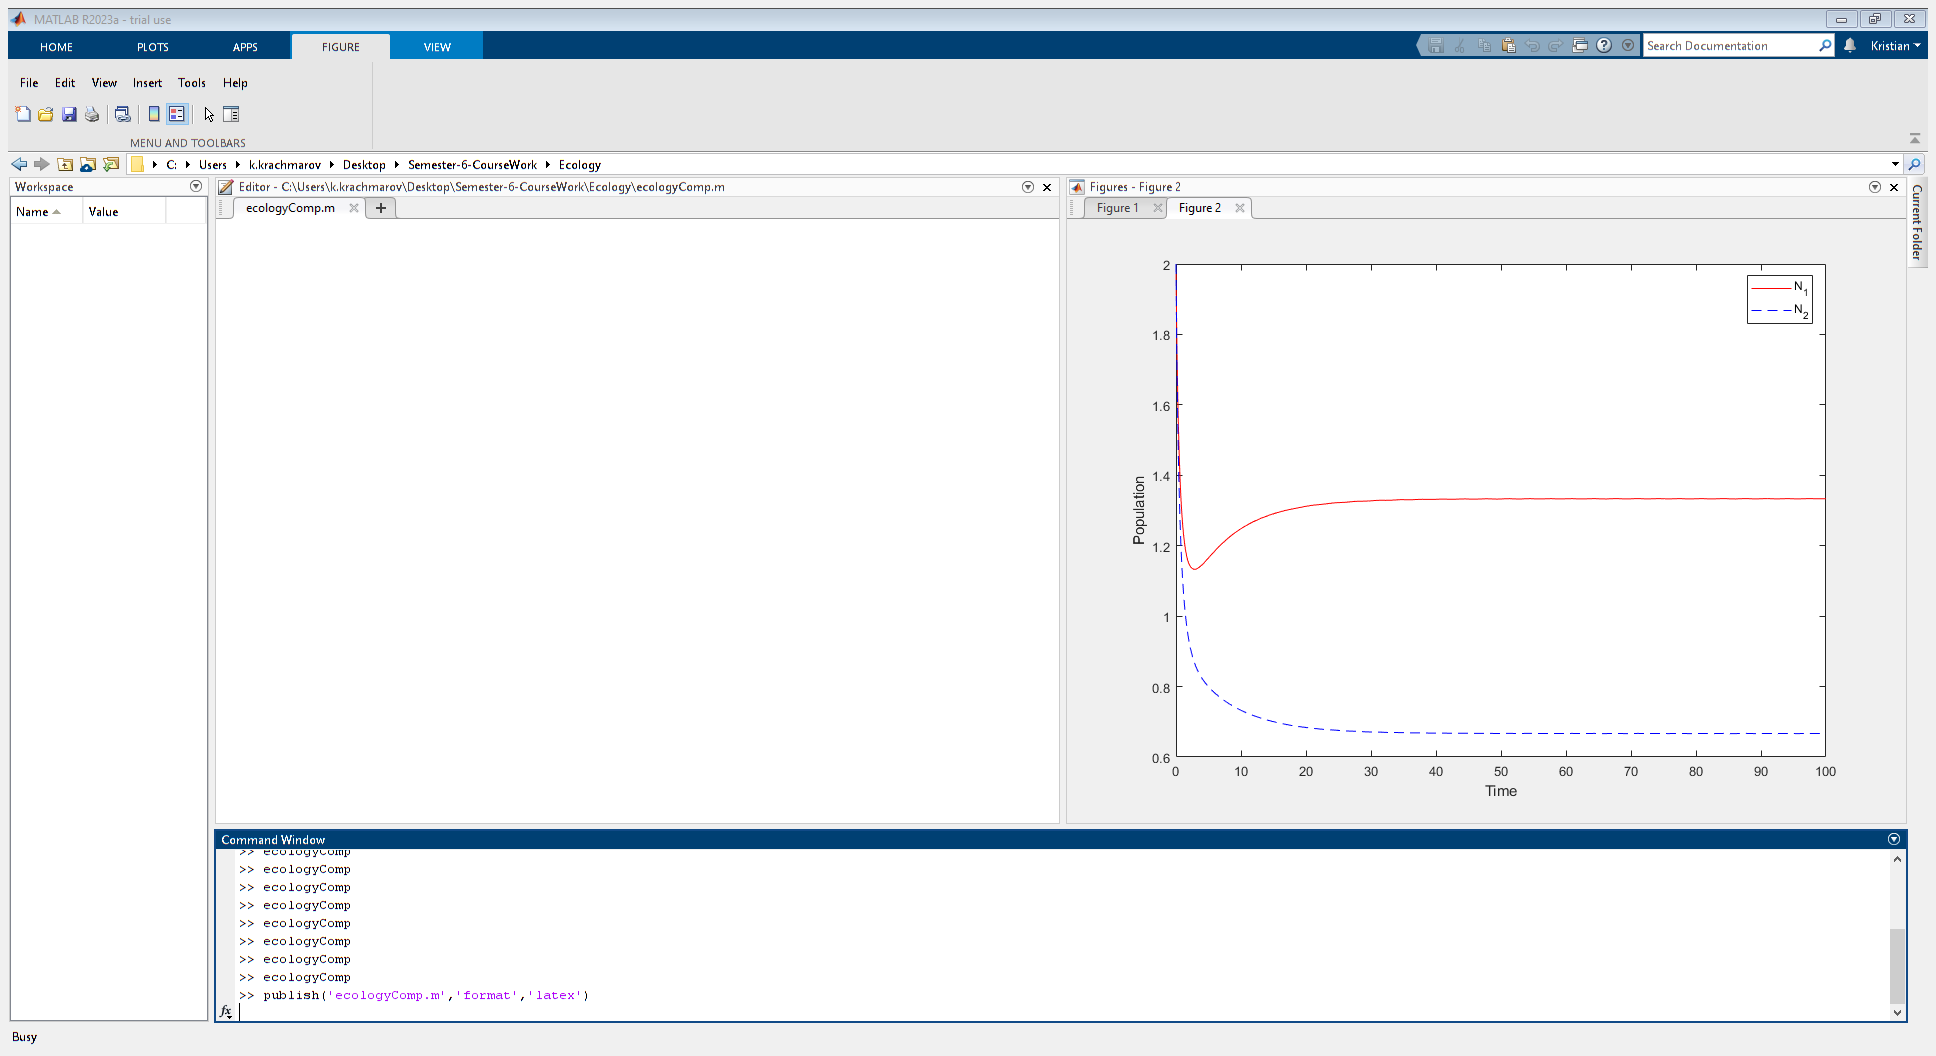
\includegraphics [width=4in]{ecologyComp_01.png}



\end{document}

